
%(BEGIN_QUESTION)
% Copyright 2008, Tony R. Kuphaldt, released under the Creative Commons Attribution License (v 1.0)
% This means you may do almost anything with this work of mine, so long as you give me proper credit

Qualitatively graph the individual proportional, integral, and derivative responses of a PID controller as it experiences a rounded ``step'' in process variable (PV):

$$\includegraphics[width=15.5cm]{i03372x01.eps}$$

Assume {\it reverse} controller action.

\vskip 20pt \vbox{\hrule \hbox{\strut \vrule{} {\bf Suggestions for Socratic discussion} \vrule} \hrule}

\begin{itemize}
\item{} Do your best to describe each action (P, I, and D) {\it verbally}, as though you are explaining each one to someone for the first time.  Keep your explanations as simple as you can without sacrificing technical accuracy.
\end{itemize}

\underbar{file i03372}
%(END_QUESTION)





%(BEGIN_ANSWER)

The controller output graph shown here is {\it qualitative} only.  Although drawn to scale (i.e. all changes in the output are properly scaled relative to each other), the scale itself is arbitrary and therefore may not match the scale of your sketch:
 
$$\includegraphics[width=15.5cm]{i03372x02.eps}$$

%(END_ANSWER)





%(BEGIN_NOTES)


%INDEX% Control: graphing proportional vs. integral vs. derivative responses

%(END_NOTES)


